\documentclass[]{article}
\usepackage{lmodern}
\usepackage{amssymb,amsmath}
\usepackage{ifxetex,ifluatex}
\usepackage{fixltx2e} % provides \textsubscript
\ifnum 0\ifxetex 1\fi\ifluatex 1\fi=0 % if pdftex
  \usepackage[T1]{fontenc}
  \usepackage[utf8]{inputenc}
\else % if luatex or xelatex
  \ifxetex
    \usepackage{mathspec}
  \else
    \usepackage{fontspec}
  \fi
  \defaultfontfeatures{Ligatures=TeX,Scale=MatchLowercase}
\fi
% use upquote if available, for straight quotes in verbatim environments
\IfFileExists{upquote.sty}{\usepackage{upquote}}{}
% use microtype if available
\IfFileExists{microtype.sty}{%
\usepackage{microtype}
\UseMicrotypeSet[protrusion]{basicmath} % disable protrusion for tt fonts
}{}
\usepackage[margin=1in]{geometry}
\usepackage{hyperref}
\hypersetup{unicode=true,
            pdftitle={A practical guide to cancer subclonal reconstruction from DNA sequencing},
            pdfborder={0 0 0},
            breaklinks=true}
\urlstyle{same}  % don't use monospace font for urls
\usepackage{color}
\usepackage{fancyvrb}
\newcommand{\VerbBar}{|}
\newcommand{\VERB}{\Verb[commandchars=\\\{\}]}
\DefineVerbatimEnvironment{Highlighting}{Verbatim}{commandchars=\\\{\}}
% Add ',fontsize=\small' for more characters per line
\usepackage{framed}
\definecolor{shadecolor}{RGB}{248,248,248}
\newenvironment{Shaded}{\begin{snugshade}}{\end{snugshade}}
\newcommand{\AlertTok}[1]{\textcolor[rgb]{0.94,0.16,0.16}{#1}}
\newcommand{\AnnotationTok}[1]{\textcolor[rgb]{0.56,0.35,0.01}{\textbf{\textit{#1}}}}
\newcommand{\AttributeTok}[1]{\textcolor[rgb]{0.77,0.63,0.00}{#1}}
\newcommand{\BaseNTok}[1]{\textcolor[rgb]{0.00,0.00,0.81}{#1}}
\newcommand{\BuiltInTok}[1]{#1}
\newcommand{\CharTok}[1]{\textcolor[rgb]{0.31,0.60,0.02}{#1}}
\newcommand{\CommentTok}[1]{\textcolor[rgb]{0.56,0.35,0.01}{\textit{#1}}}
\newcommand{\CommentVarTok}[1]{\textcolor[rgb]{0.56,0.35,0.01}{\textbf{\textit{#1}}}}
\newcommand{\ConstantTok}[1]{\textcolor[rgb]{0.00,0.00,0.00}{#1}}
\newcommand{\ControlFlowTok}[1]{\textcolor[rgb]{0.13,0.29,0.53}{\textbf{#1}}}
\newcommand{\DataTypeTok}[1]{\textcolor[rgb]{0.13,0.29,0.53}{#1}}
\newcommand{\DecValTok}[1]{\textcolor[rgb]{0.00,0.00,0.81}{#1}}
\newcommand{\DocumentationTok}[1]{\textcolor[rgb]{0.56,0.35,0.01}{\textbf{\textit{#1}}}}
\newcommand{\ErrorTok}[1]{\textcolor[rgb]{0.64,0.00,0.00}{\textbf{#1}}}
\newcommand{\ExtensionTok}[1]{#1}
\newcommand{\FloatTok}[1]{\textcolor[rgb]{0.00,0.00,0.81}{#1}}
\newcommand{\FunctionTok}[1]{\textcolor[rgb]{0.00,0.00,0.00}{#1}}
\newcommand{\ImportTok}[1]{#1}
\newcommand{\InformationTok}[1]{\textcolor[rgb]{0.56,0.35,0.01}{\textbf{\textit{#1}}}}
\newcommand{\KeywordTok}[1]{\textcolor[rgb]{0.13,0.29,0.53}{\textbf{#1}}}
\newcommand{\NormalTok}[1]{#1}
\newcommand{\OperatorTok}[1]{\textcolor[rgb]{0.81,0.36,0.00}{\textbf{#1}}}
\newcommand{\OtherTok}[1]{\textcolor[rgb]{0.56,0.35,0.01}{#1}}
\newcommand{\PreprocessorTok}[1]{\textcolor[rgb]{0.56,0.35,0.01}{\textit{#1}}}
\newcommand{\RegionMarkerTok}[1]{#1}
\newcommand{\SpecialCharTok}[1]{\textcolor[rgb]{0.00,0.00,0.00}{#1}}
\newcommand{\SpecialStringTok}[1]{\textcolor[rgb]{0.31,0.60,0.02}{#1}}
\newcommand{\StringTok}[1]{\textcolor[rgb]{0.31,0.60,0.02}{#1}}
\newcommand{\VariableTok}[1]{\textcolor[rgb]{0.00,0.00,0.00}{#1}}
\newcommand{\VerbatimStringTok}[1]{\textcolor[rgb]{0.31,0.60,0.02}{#1}}
\newcommand{\WarningTok}[1]{\textcolor[rgb]{0.56,0.35,0.01}{\textbf{\textit{#1}}}}
\usepackage{longtable,booktabs}
\usepackage{graphicx,grffile}
\makeatletter
\def\maxwidth{\ifdim\Gin@nat@width>\linewidth\linewidth\else\Gin@nat@width\fi}
\def\maxheight{\ifdim\Gin@nat@height>\textheight\textheight\else\Gin@nat@height\fi}
\makeatother
% Scale images if necessary, so that they will not overflow the page
% margins by default, and it is still possible to overwrite the defaults
% using explicit options in \includegraphics[width, height, ...]{}
\setkeys{Gin}{width=\maxwidth,height=\maxheight,keepaspectratio}
\IfFileExists{parskip.sty}{%
\usepackage{parskip}
}{% else
\setlength{\parindent}{0pt}
\setlength{\parskip}{6pt plus 2pt minus 1pt}
}
\setlength{\emergencystretch}{3em}  % prevent overfull lines
\providecommand{\tightlist}{%
  \setlength{\itemsep}{0pt}\setlength{\parskip}{0pt}}
\setcounter{secnumdepth}{0}
% Redefines (sub)paragraphs to behave more like sections
\ifx\paragraph\undefined\else
\let\oldparagraph\paragraph
\renewcommand{\paragraph}[1]{\oldparagraph{#1}\mbox{}}
\fi
\ifx\subparagraph\undefined\else
\let\oldsubparagraph\subparagraph
\renewcommand{\subparagraph}[1]{\oldsubparagraph{#1}\mbox{}}
\fi

%%% Use protect on footnotes to avoid problems with footnotes in titles
\let\rmarkdownfootnote\footnote%
\def\footnote{\protect\rmarkdownfootnote}

%%% Change title format to be more compact
\usepackage{titling}

% Create subtitle command for use in maketitle
\providecommand{\subtitle}[1]{
  \posttitle{
    \begin{center}\large#1\end{center}
    }
}

\setlength{\droptitle}{-2em}

  \title{A practical guide to cancer subclonal reconstruction from DNA sequencing}
    \pretitle{\vspace{\droptitle}\centering\huge}
  \posttitle{\par}
    \author{}
    \preauthor{}\postauthor{}
      \predate{\centering\large\emph}
  \postdate{\par}
    \date{28 February 2020}

\usepackage{caption} \usepackage{float}

\floatplacement{figure}{H}
\captionsetup[figure]{labelfont={bf},name={Figure}, labelsep=period}

\begin{document}
\maketitle

{
\setcounter{tocdepth}{2}
\tableofcontents
}
\newpage

\hypertarget{introduction}{%
\section{Introduction}\label{introduction}}

\hypertarget{about-this-guide}{%
\subsection{About this guide}\label{about-this-guide}}

In this guide we will go through the steps of reconstructing a tumour
subclonal architecture (\textbf{Figure\ref{Figure1}A}). For simplicity,
we will be starting from one pair of patient-matched simulated tumour
and normal bam files.

These bam files have been simulated using
\href{https://github.com/adamewing/bamsurgeon}{\textbf{BAMSurgeon}} to
correspond to a pre-designed tumour phylogeny shown on
\textbf{Figure\ref{Figure1}B}. Knowing the true mutations, copy number
aberrations and underlying subclonal structure will help illustrate and
give maximal insight into the concepts at each step of the pipeline.

\begin{figure}[H]
  \centering
  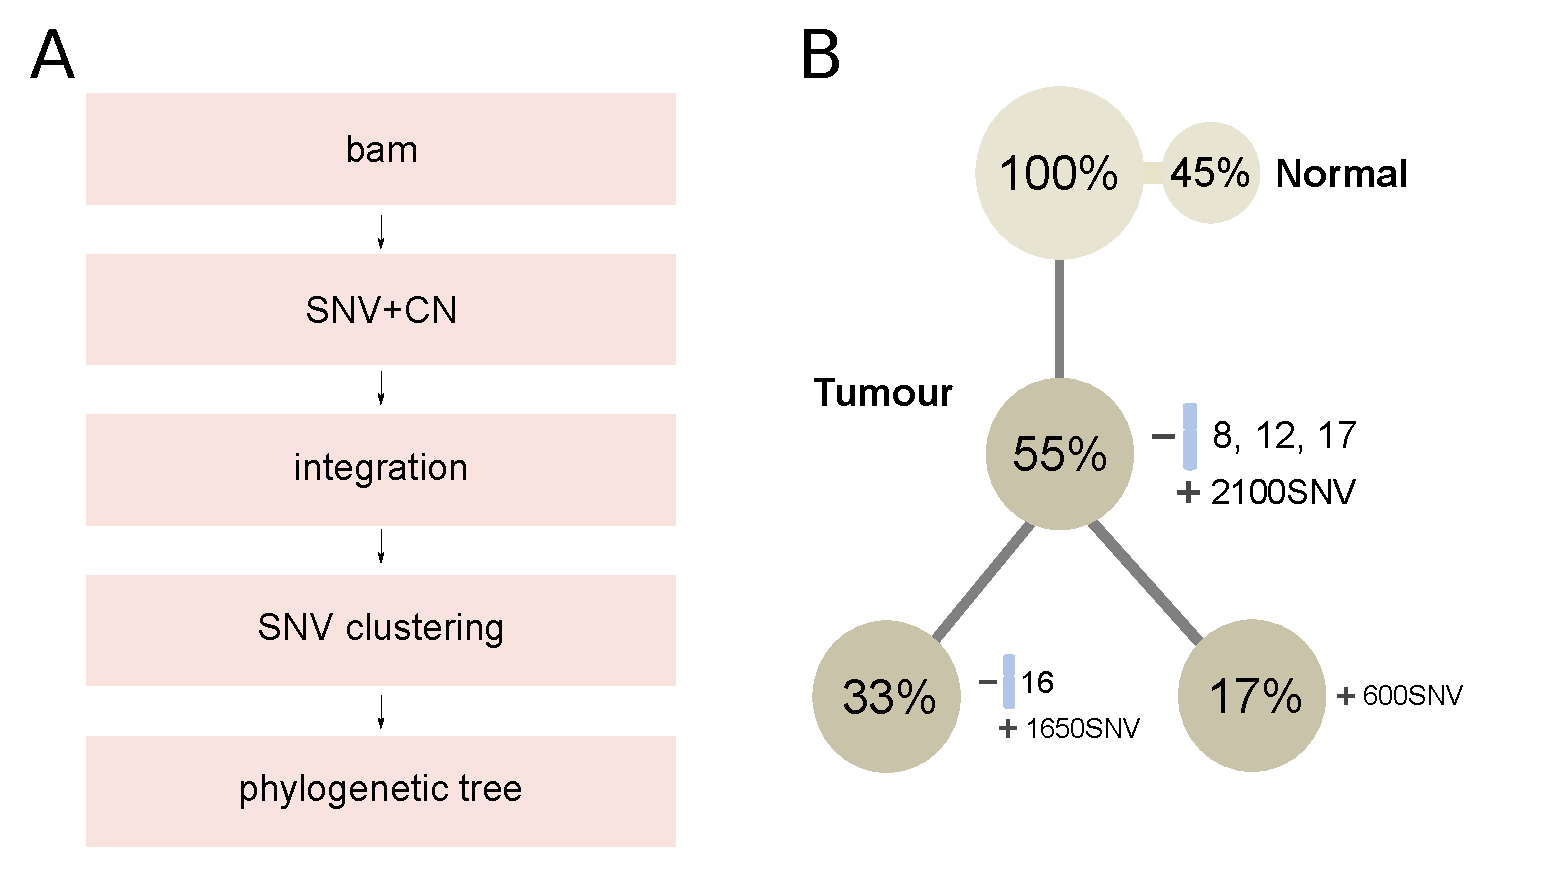
\includegraphics{figures/fig1_pipelineOutline.pdf}
  \caption{A. Pipeline outline. We will go through each step in this
  guide. B. Simulated tumour phylogeny. A few thousands SNV, 3 lost
  chromosome clonally and one lost chromosome subclonally. 
  The simulated BAM, vcf and copy number outputs are available
  for download (see next section).}
  \label{Figure1}
\end{figure}

For each step of the SRC, we have chosen one method for illustration
purposes. However, the choice of the methods should be carefully
considered by the user. Indeed, different methods will have different
behaviour and might be better suited for the type of samples or project
at hand. In the main text, we only recommend methods with specific
characteristics, e.g.~take into account copy number, Beta or Binomial
models, picking one/the best method is not the subject of this guide.

Although, we will cover some of the theoretical aspects of the different
methods and SRC in this practical guide, we recommend a more in-depth
book chapter on the principles of SRC by Dentro, Wedge, and Van Loo
(Dentro, Wedge, and Van Loo 2017).

\hypertarget{availability}{%
\subsection{Availability}\label{availability}}

This guide is also available on github:
\textbf{\url{https://github.com/galder-max/src_guide}}. The data used
here is available online, see next section for details. For each method,
we provide hyperlink to their online webpage.

\newpage

\hypertarget{download-input-data}{%
\section{Download input data}\label{download-input-data}}

Important note: There is no need to start from the BAM file. If you
would like to skip some of the steps upstream of the clustering and
phylogeny inference, all the input files are already available online on
synapse (see following section).

\hypertarget{input-bam-file}{%
\subsection{Input BAM file}\label{input-bam-file}}

The input BAM files were generated as part of another project (Salcedo
et al. 2020) and can be downloaded from EGA under study accession no.
\href{https://www.ebi.ac.uk/ega/studies/EGAS00001002092}{\textbf{EGAD00001003971}}.

\hypertarget{vcf-files}{%
\subsection{VCF files}\label{vcf-files}}

It will be less time consuming to start form vcf files. Mutation calling
has already been performed with four different callers on these BAMs. In
this guide we will use the ``perfect'' or ``true'' calls, i.e.~the
mutations as input to the simulator, and compare them to the MuTect
calls. All vcf files are available on
\href{https://www.synapse.org/\#!Synapse:syn2813581/wiki/303137}{\textbf{synapse}}.
The vcf files accession number is syn21609786. Here we will be using T2
at 128X, the file is named \emph{perfect\_T2.T.128X\_noXY.vcf}. We will
compare the results with results obtained on downsampled BAM files at
half the depth, i.e.~64X. These files are also available in the same
tarball, together with 32X, 16X and 8X.

\hypertarget{copy-number-aberration-calling}{%
\subsection{Copy number aberration
calling}\label{copy-number-aberration-calling}}

CNA calling has been performed using
\href{https://github.com/Wedge-Oxford/battenberg}{\textbf{Battenberg}}
(Nik-Zainal et al. 2012). The output files can be downloadded in synapse
with accession number syn21609785. Again, we are using T2 at 128X. The
files are named \emph{T2-128X\_refit\_cellularity\_ploidy.txt} and
\emph{T2-128X\_refit\_subclones\_noXY.txt}. The former contains the
purity and ploidy values, while the latter contains the per segment copy
number calls. Battenberg outputs for downsampled BAM files are also
available at 64X, 32X, 16X and 8X.

\newpage

\hypertarget{step-by-step-guide}{%
\section{Step-by-step guide}\label{step-by-step-guide}}

\hypertarget{alignment-with-bwa-mem}{%
\subsection{Alignment with BWA-mem}\label{alignment-with-bwa-mem}}

We will assume that most quality checks have been performed and the
first step after receiving your sequences fresh from the sequencing
facility, is to align the fastq files to the reference genome. Here we
have used
\href{http://ftp.1000genomes.ebi.ac.uk/vol1/ftp/technical/reference/phase2_reference_assembly_sequence/hs37d5.fa.gz}{\textbf{hg19}}
and aligned with \href{https://github.com/lh3/bwa}{\textbf{BWA-mem}} (Li
2013).

You might also want to consider read trimming and further processing of
the alignmed BAM for variant calling such as realignment around indels
and base recalibration. Mutation callers will usually include these
steps in their pipeline documentation.

\hypertarget{mutation-calling}{%
\subsection{Mutation calling}\label{mutation-calling}}

Mutation calling is a complex classification task where the whole tumour
BAM file is compared to the normal BAM file, differences have to be
picked up and characterised, and finally each difference has to be
classified as either a true somatic change or a technical artefact.

For the clustering and SRC, we are starting from the substitutions, or
single nucleotide variants (SNVs). Many algorithms have been proposed to
call SNVs. Some perform better than others but the current good practice
is to combined multiple callers into a consensus (Ewing et al. 2015),
typically with a majority vote strategy, e.g.~considering true variant
if called by 2 out of 3 callers.

\hypertarget{typical-run-with-a-previous-version-of-mutect}{%
\subsubsection{Typical run with (a previous version of)
MuTect}\label{typical-run-with-a-previous-version-of-mutect}}

Here, to illustrate a typical run, we show how a previous version of
MuTect was run to generate the
\href{https://software.broadinstitute.org/cancer/cga/mutect_download}{\textbf{MuTect}}
(Cibulskis et al. 2013) MuTect vcf files.

\begin{Shaded}
\begin{Highlighting}[]
\KeywordTok{print}\NormalTok{(cmd)}
\end{Highlighting}
\end{Shaded}

\begin{verbatim}
## [1] "java -Xmx8g -jar muTect-1.1.4.jar -T MuTect --tumor_lod 10 --tumor_sample_name T2
--normal_sample_name HG002 --reference_sequence hs37d5.fa --cosmic cosmic.header.vcf
--dbsnp dbsnp.nochr.vcf --input_file:normal HG002.N.bam --input_file:tumor T2.T.128X.bam
--out outFile.out --vcf outVcf.vcf --coverage_file outCoverage.wig"
\end{verbatim}

On new data,
\href{https://gatk.broadinstitute.org/hc/en-us/articles/360037593851-Mutect2}{MuTect2},
which also allows to run on multiple samples, should be preferred over
MuTect.

\hypertarget{false-positives-at-low-vaf}{%
\subsubsection{False positives at low
VAF}\label{false-positives-at-low-vaf}}

Now, let's load the MuTect and perfect vcf files and compare them. We
will compare the mutation calls as well as the distribution of variant
allele frequencies (VAF), i.e.~fraction of mutated reads.

We will use a simple read.table function for minimal dependencies, but
more sophisticated read functions are available for vcf files (e.g.
\emph{readVcf} from package \emph{VariantAnnotation}).

\begin{Shaded}
\begin{Highlighting}[]
\NormalTok{vcf_perfect <-}\StringTok{ }\KeywordTok{read.table}\NormalTok{(}\StringTok{"input/perfect_T2.T.128X_noXY.vcf"}\NormalTok{,}\DataTypeTok{sep=}\StringTok{"}\CharTok{\textbackslash{}t}\StringTok{"}\NormalTok{)}
\KeywordTok{head}\NormalTok{(vcf_perfect)}
\end{Highlighting}
\end{Shaded}

\begin{verbatim}
##   V1      V2 V3 V4 V5  V6   V7                                     V8 V9
## 1  1  556789  .  T  A 100 PASS   SOMATIC;VAF=0.118279569892473;DPR=93 AD
## 2  1  763107  .  C  T 100 PASS               SOMATIC;VAF=0.25;DPR=180 AD
## 3  1  946288  .  C  T 100 PASS  SOMATIC;VAF=0.241610738255034;DPR=149 AD
## 4  1 1358216  .  C  T 100 PASS  SOMATIC;VAF=0.291666666666667;DPR=144 AD
## 5  1 1375339  .  C  T 100 PASS  SOMATIC;VAF=0.280701754385965;DPR=114 AD
## 6  1 2801021  .  T  C 100 PASS SOMATIC;VAF=0.0814814814814815;DPR=135 AD
##      V10
## 1  82,11
## 2 134,45
## 3 110,36
## 4 101,42
## 5  81,32
## 6 124,11
\end{verbatim}

\begin{Shaded}
\begin{Highlighting}[]
\NormalTok{vcf_mutect <-}\StringTok{ }\KeywordTok{read.table}\NormalTok{(}\StringTok{"input/mutect_T2.T.128X_noXY.vcf"}\NormalTok{,}\DataTypeTok{sep=}\StringTok{"}\CharTok{\textbackslash{}t}\StringTok{"}\NormalTok{)}
\KeywordTok{head}\NormalTok{(vcf_mutect)}
\end{Highlighting}
\end{Shaded}

\begin{verbatim}
##   V1      V2          V3 V4 V5 V6   V7                V8                V9
## 1  1  763080 rs189703925  G  T  . PASS DB;SOMATIC;VT=SNP GT:AD:BQ:DP:FA:SS
## 2  1  763107           .  C  T  . PASS    SOMATIC;VT=SNP GT:AD:BQ:DP:FA:SS
## 3  1  831651  rs28864374  A  G  . PASS DB;SOMATIC;VT=SNP GT:AD:BQ:DP:FA:SS
## 4  1  946288           .  C  T  . PASS    SOMATIC;VT=SNP GT:AD:BQ:DP:FA:SS
## 5  1 1358216           .  C  T  . PASS    SOMATIC;VT=SNP GT:AD:BQ:DP:FA:SS
## 6  1 1375339           .  C  T  . PASS    SOMATIC;VT=SNP GT:AD:BQ:DP:FA:SS
##                         V10                       V11
## 1       0:80,1:.:81:0.012:0  0/1:150,7:38:157:0.045:2
## 2        0:89,0:.:89:0.00:0 0/1:130,45:32:175:0.257:2
## 3 0:101,1:.:102:9.804e-03:0  0/1:148,7:37:155:0.045:2
## 4       0:98,0:.:100:0.00:0  0/1:98,30:31:128:0.234:2
## 5        0:75,0:.:75:0.00:0  0/1:99,41:34:140:0.293:2
## 6        0:96,0:.:96:0.00:0  0/1:78,32:34:110:0.291:2
\end{verbatim}

As we can see, some of the fields look similar, and are usually the
mandatory vcf fields, while others are formatted differently. This is
documented in the vcf header.

First we look at the chromosomal positions and the associated base
changes and compare them between the two set of calls.

\begin{Shaded}
\begin{Highlighting}[]
\NormalTok{mut_perfect <-}\StringTok{ }\KeywordTok{do.call}\NormalTok{(}\ControlFlowTok{function}\NormalTok{(...) }\KeywordTok{paste}\NormalTok{(...,}\DataTypeTok{sep=}\StringTok{":"}\NormalTok{),}
                       \KeywordTok{lapply}\NormalTok{(}\KeywordTok{c}\NormalTok{(}\DecValTok{1}\NormalTok{,}\DecValTok{2}\NormalTok{,}\DecValTok{4}\NormalTok{,}\DecValTok{5}\NormalTok{),}\ControlFlowTok{function}\NormalTok{(x) vcf_perfect[,x]))}
\NormalTok{mut_mutect <-}\StringTok{ }\KeywordTok{do.call}\NormalTok{(}\ControlFlowTok{function}\NormalTok{(...) }\KeywordTok{paste}\NormalTok{(...,}\DataTypeTok{sep=}\StringTok{":"}\NormalTok{),}
                      \KeywordTok{lapply}\NormalTok{(}\KeywordTok{c}\NormalTok{(}\DecValTok{1}\NormalTok{,}\DecValTok{2}\NormalTok{,}\DecValTok{4}\NormalTok{,}\DecValTok{5}\NormalTok{),}\ControlFlowTok{function}\NormalTok{(x) vcf_mutect[,x]))}
\KeywordTok{list}\NormalTok{(}\DataTypeTok{count_perfect=}\KeywordTok{length}\NormalTok{(mut_perfect),}
     \DataTypeTok{count_mutect=}\KeywordTok{length}\NormalTok{(mut_mutect),}
     \DataTypeTok{count_intersect=}\KeywordTok{length}\NormalTok{(}\KeywordTok{intersect}\NormalTok{(mut_perfect,mut_mutect)))}
\end{Highlighting}
\end{Shaded}

\begin{verbatim}
## $count_perfect
## [1] 4062
## 
## $count_mutect
## [1] 4374
## 
## $count_intersect
## [1] 3827
\end{verbatim}

So we see that mutect has missed a few mutations while calling a few
extra ones as well. Typically, these false positives display low VAF, so
let's verify this.

The perfect calls store the tumour VAFs in the 8th column, while mutect
calls store the tumour VAFs in the 11th column (named \emph{tumor}) in
the FA field. There are many ways to go about extracting this
information. Here, we will use simple regular expression searches.

\begin{Shaded}
\begin{Highlighting}[]
\NormalTok{vaf_perfect <-}\StringTok{ }\KeywordTok{as.numeric}\NormalTok{(}\KeywordTok{gsub}\NormalTok{(}\StringTok{"(.*);VAF=(.*);DPR=(.*)"}\NormalTok{,}\StringTok{"}\CharTok{\textbackslash{}\textbackslash{}}\StringTok{2"}\NormalTok{,vcf_perfect[,}\DecValTok{8}\NormalTok{]))}
\NormalTok{vaf_mutect <-}\StringTok{ }\KeywordTok{as.numeric}\NormalTok{(}\KeywordTok{gsub}\NormalTok{(}\StringTok{"(.*):(.*):(.*):(.*):(.*):(.*)"}\NormalTok{,}\StringTok{"}\CharTok{\textbackslash{}\textbackslash{}}\StringTok{5"}\NormalTok{,vcf_mutect[,}\DecValTok{11}\NormalTok{]))}
\end{Highlighting}
\end{Shaded}

\begin{Shaded}
\begin{Highlighting}[]
\KeywordTok{head}\NormalTok{(vaf_perfect)}
\end{Highlighting}
\end{Shaded}

\begin{verbatim}
## [1] 0.11827957 0.25000000 0.24161074 0.29166667 0.28070175 0.08148148
\end{verbatim}

We can then plot the histograms of VAF and compare MuTect to simulated.

\begin{figure}

{\centering 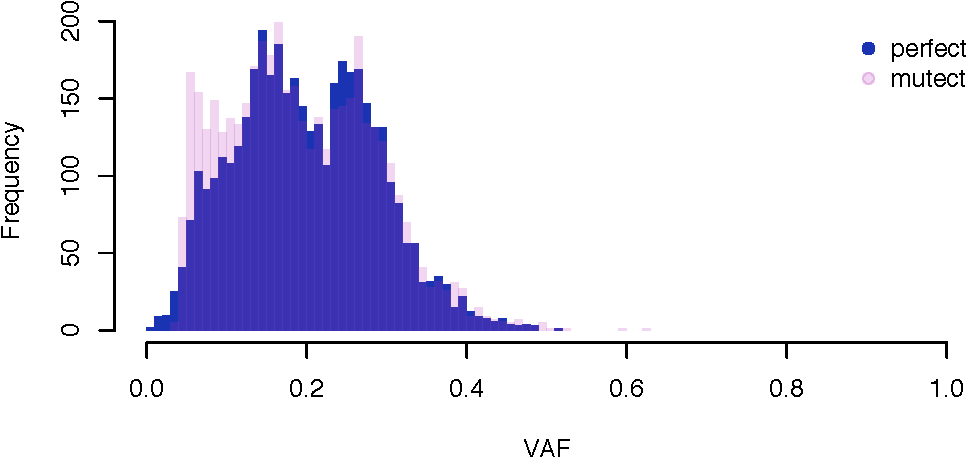
\includegraphics{src_guide_files/figure-latex/fig1-1} 

}

\caption{\label{fig1}Variant allele frequency distributions: MuTect vs. simulated}\label{fig:fig1}
\end{figure}

As expected, MuTect has called extra mutations at low allele
frequencies.

\hypertarget{effect-of-read-depth-on-the-vaf-distribution}{%
\subsubsection{Effect of read depth on the VAF
distribution}\label{effect-of-read-depth-on-the-vaf-distribution}}

One can downsample a BAM file, i.e.~keep only a fraction of the reads
and these need to be randomly sampled. SAMtools has a function for this
that makes this really easy, see \emph{samtools view -s}. Here, we will
use the pre-computed vcf files on the downsampled BAM file. We load the
vcf derived at 32X and the vcf derived at 128X and compare their VAF
distribution.

\begin{Shaded}
\begin{Highlighting}[]
\NormalTok{vcf_perfect_32X <-}\StringTok{ }\KeywordTok{read.table}\NormalTok{(}\StringTok{"input/perfect_T2.T.32X_noXY.vcf"}\NormalTok{,}\DataTypeTok{sep=}\StringTok{"}\CharTok{\textbackslash{}t}\StringTok{"}\NormalTok{)}
\NormalTok{vaf_perfect_32X <-}\StringTok{ }\KeywordTok{as.numeric}\NormalTok{(}\KeywordTok{gsub}\NormalTok{(}\StringTok{"(.*);VAF=(.*);DPR=(.*)"}\NormalTok{,}\StringTok{"}\CharTok{\textbackslash{}\textbackslash{}}\StringTok{2"}\NormalTok{,vcf_perfect_32X[,}\DecValTok{8}\NormalTok{]))}
\end{Highlighting}
\end{Shaded}

\begin{figure}

{\centering 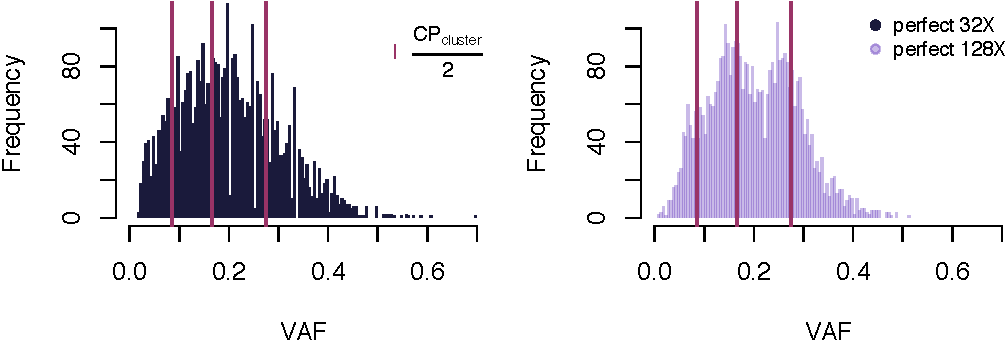
\includegraphics{src_guide_files/figure-latex/fig1b-1} 

}

\caption{\label{fig1b}Variant allele frequency distributions: Simulated 32X vs. simulated 128X. Flattening of the VAF distribution at lower depth. Vertical lines show the cellular prevalence of the subclone divided by 2. That is where the VAF peak is expected for mutation falling in diploid regions.}\label{fig:fig1b}
\end{figure}

\newpage

\hypertarget{copy-number-calling-with-battenberg}{%
\subsection{Copy number calling with
Battenberg}\label{copy-number-calling-with-battenberg}}

We have run
\href{https://github.com/Wedge-Oxford/battenberg}{\textbf{Battenberg}}
to call copy number aberrations and flag subclonal segments. If you
would like to run it as well, please follow the documentation on the
\href{https://github.com/Wedge-Oxford/battenberg}{\textbf{github page}}
to install and run it.

\hypertarget{how-does-it-work}{%
\subsubsection{How does it work}\label{how-does-it-work}}

To call subclonal copy number aberrations we will use an algorithm
called Battenberg, which was originally published by Nik-Zainal and
colleagues (Nik-Zainal et al. 2012). Battenberg methodology and
algorithm are based on the code and equations of ASCAT (Van Loo et al.
2010) to simultaneously derive purity and ploidy of tumour samples and
call allele-specific clonal CNAs.

Briefly, to infer ploidy \(\psi\) and purity \(\rho\) of the samples,
ASCAT looks at how the logR \(r_i\) and the bi-allelic frequency (BAF)
\(b_i\) of heterozygous SNPs are influenced by copy-number-induced
allelic imbalances across the genome; as a consequence ASCAT will fail
to report estimates for cancer genomes presenting no allelic imbalances,
which is a rare case for cancers but not the expection for less advanced
or benign tumours.

Then to call CNAs given a sample's purity and ploidy, ASCAT solves a
system of two equations with two unkowns formed by writing LogR and BAF
of heterozygous SNPs as a function of the number of copies of allele A
\(N_A\) and number of copies of allele B \(N_B\):

\[\begin{array}{lcl} r_i&=&
  log_2(\frac{2(1-\rho)+\rho(N_{A,i}+N_{B,i})}{\psi})\\ b_i&=&\frac{1-\rho+\rho N_{B,i}}{2-2\rho+\rho(N_{A,i}+N_{B,i})}
\end{array}\]

Where \(\rho\) is the purity and \(\psi\) is the average tissue ploidy.

To remove noise only the BAF track is segmented using piecewise constant
fitting (Van Loo et al. 2010).

A grid search is then used to find the pair of realistic purity and
ploidy values that minimises the genome-wide error between observed and
expected \(N_A\) and \(N_B\) values. The expected \(N_A\) and \(N_B\)
are approximated by rounding the observed \(N_A\) and \(N_B\) to the
closest integers.

Battenberg runs this clonal version of ASCAT and then infers subclonal
regions by looking at significant deviations of BAF of heterozygous SNPs
from the expected BAF of clonal states. If deviations are significant,
Battenberg flags the segment as subclonal. However, the subclonal states
are not trivially obtained from the logR and the BAF, as there are now
more unkowns than equations.

Using heuristics, Battenberg outputs a few possible solutions, i.e.~up
to 6 pairs of integer copy number states and their associated cancer
cell fractions. For example, 1+1 in 70\% cancer cells and 2+1 in 30\%
cancer cells would translate into: 70\% of cancer cells carrying 1 copy
of each allele, and 30\% of cancer cells carrying 2 copies of the major
allele and 1 copy of the minor allele. These pairs of states are chosen
to be mixed states differing by one or two losses or gains from the
closest clonal state that would correspond to the observed logR and BAF.
The states are taken as combinations of integer states. Once the two
mixed states are fixed, the cancer cell fractions (CCFs) (\(\tau\) and
\(1-\tau\)) of these states \((N_{A,1}+N_{B,1}) \& (N_{A,2}+N_{B,2})\)
can be inferred from observed average BAF across the genomic segment
\(b_s\):

\[ \tau=\frac{1-\rho+\rho
  N_{B,2}-2b_s(1-\rho)-b_s\rho(N_{A,2}+N_{B,2})}{b_s\rho(N_{A,1}+N_{B,1})-b_s\rho(N_{A,2}+N_{B,2})-\rho
  N_{B,1}+\rho N_{B,2}}\]

What is more Battenberg uses haplotyped SNPs to increase its sensitivity
to detect the BAF deviations from expected BAF of clonal states. The
haplotypes are imputed using impute2 (Howie, Donnelly, and Marchini
2009) and a two-step segmentation stragegy of the BAF track helps take
advantage of these imputed haplotypes. Briefly, haplotyped SNPs
translate into phased BAF values, but also include switching errors.
Therefore first the phased BAF track is segmented using a very sensitive
segmentation. This identifies haplotypes and longer phased blocks. Then
BAF values are mirrored per segment to have a segment average above 0.5,
i.e.~if(average(BAF)\textless{}0.5) BAF=1-BAF. Finally, a more specific
segmentation is run to obtain the final segments.

The last step is to go through each segment's BAF and LogR to call the
segment state(s), as described above.

\hypertarget{how-does-it-look}{%
\subsubsection{How does it look}\label{how-does-it-look}}

First we note that the Battenberg profile is named \emph{refit}. This
indicates that the default fit was not a good one and manual inspection
and refitting were necessary. Below we show the default fit found by
Battenberg and the refitted profile.

\begin{figure}[H]
  \centering
  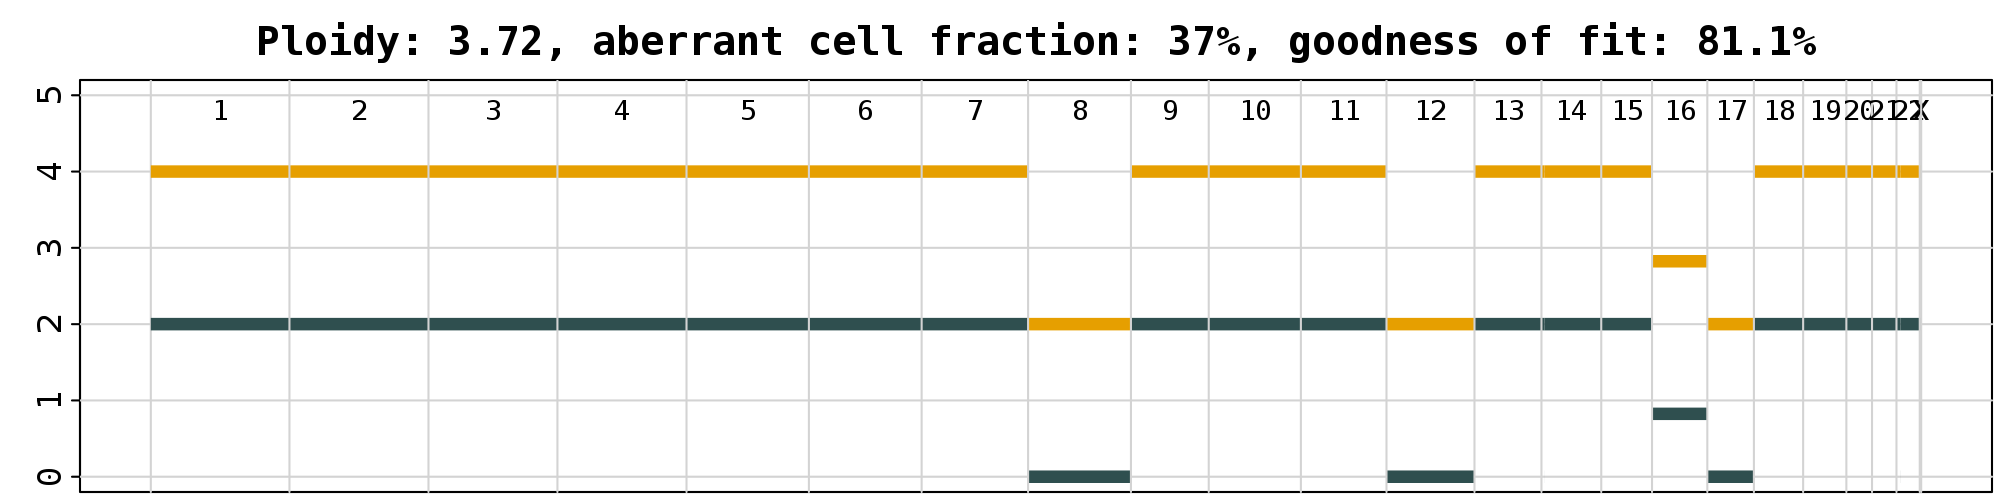
\includegraphics{figures/T2-128X_BattenbergProfile_average.png}
  \caption{\textbf{Battenberg default profile.} Along the genome on the x-axis,
  copy number of the minor (dark blue) and total (orange) per chromosome.}
  \label{Figure4}
\end{figure}

\begin{figure}[H]
  \centering
  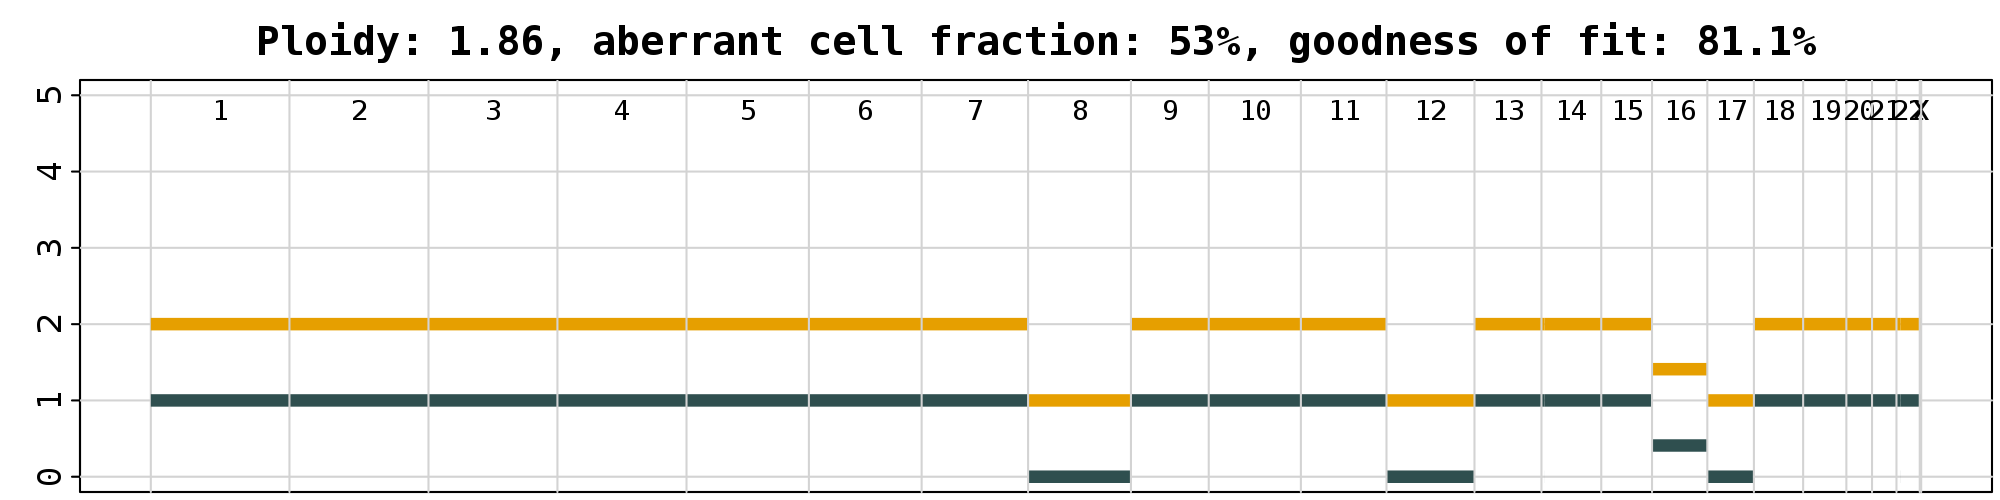
\includegraphics{figures/T2-128X_BattenbergProfile.refit_average.png}
  \caption{\textbf{Battenberg refitted profile.} Along the genome on the x-axis,
  copy number of the minor (dark blue) and total (orange) per chromosome.}
  \label{Figure5}
\end{figure}

This is a good illustration of the ambiguity of \emph{in silico} ploidy
estimates. The default fit proposes twice the actual ploidy. This is
likely because of the subclonal loss on chromosome 16 which is almost at
50\% of the main clone CP, which brings this segment closer to an
integer in the whole-genome duplicated fit.

After the manual refit, the ploidy and the purity better match the
simulation design.

The previous figures are generated by Battenberg. We can also derive
them ourselves from the copy number profile. Now we load the Battenberg
CNA profile -we only keep the first thirteen columns-, which include
only one of the possible solutions for subclonal segments. Then we plot
the genomewide profile.

\begin{Shaded}
\begin{Highlighting}[]
\NormalTok{cna_bb <-}\StringTok{ }\KeywordTok{read.table}\NormalTok{(}\StringTok{"input/T2-128X_refit_subclones_noXY.txt"}\NormalTok{,}\DataTypeTok{sep=}\StringTok{"}\CharTok{\textbackslash{}t}\StringTok{"}\NormalTok{,}\DataTypeTok{header=}\NormalTok{T)[,}\DecValTok{1}\OperatorTok{:}\DecValTok{13}\NormalTok{]}
\KeywordTok{head}\NormalTok{(cna_bb)}
\end{Highlighting}
\end{Shaded}

\begin{verbatim}
##   chr startpos    endpos       BAF pval       LogR     ntot nMaj1_A
## 1   1   811735 249223191 0.5013481    1 0.04334820 2.008582       1
## 2   2    23368 242985695 0.5011866    1 0.04252642 2.006444       1
## 3   3    60596 197846280 0.5011744    1 0.04301515 2.007715       1
## 4   4   109541 190781263 0.5010340    1 0.04298700 2.007642       1
## 5   5   859234 180742812 0.5013670    1 0.04378574 2.009720       1
## 6   6   203397 170898626 0.5012337    1 0.04301005 2.007702       1
##   nMin1_A frac1_A nMaj2_A nMin2_A frac2_A
## 1       1       1      NA      NA      NA
## 2       1       1      NA      NA      NA
## 3       1       1      NA      NA      NA
## 4       1       1      NA      NA      NA
## 5       1       1      NA      NA      NA
## 6       1       1      NA      NA      NA
\end{verbatim}

The columns indicate the chromosome, start, end of the segments, their
average BAF, p-value of being subclonal (i.e.~non-integer given the
purity ahd ploidy values), the LogR, the non-rounded total copies, the
number of copies of the major allele, and the minor allele and the
fraction of cells in which these states are present. If subclonal the
segment is detected as subclonal, the latter is lower than 1 and a
second copy number state is given together with the fraction of cancer
cells in which it is present. There is too much ambiguity in those
states, and while these states are not consistent across CNA methods,
CNA methods usually agree on whether the segment should be deemed
subclonal.

Now, let's visualise the total and minor copies along the genome.

\begin{figure}

{\centering 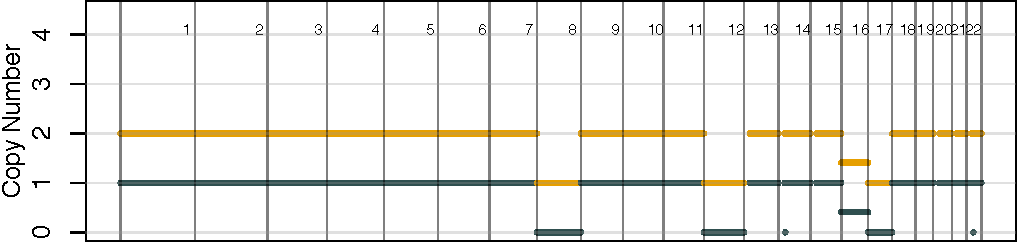
\includegraphics{src_guide_files/figure-latex/fig2-1} 

}

\caption{\label{fig2} Battenberg plot from the input file. Along the genome on the x-axis, copy number of the minor (dark blue) and total (orange) per chromosome. }\label{fig:fig2}
\end{figure}

Importantly, this figure is showing genomic position on the x-axis while
the Battenberg figures are showing SNP index. The latter is very useful
to visualise relative number of SNPs per chromosome and identify
characteristics of the run, such as long stretches of homozygosity,
often seen in inbred population. This stretches are blindspots for
segmentation with Battenberg, which is based solely on the BAF of
heterozygous SNPs.

\hypertarget{impact-of-read-depth-on-cna}{%
\subsubsection{Impact of read depth on
CNA}\label{impact-of-read-depth-on-cna}}

The VAF of a given SNV is influenced the tumour purity and its number of
bearing copies. The noise on the VAF estimate is pretty much directly
defined by the read depth, which can be a limiting factor.

For copy number, the length of the implicated segment comes into play as
well. Large copy number events can be picked up in single cells with
coverage as low as 0.1X.

So far, there has been no consistent benchmarking of methods for copy
number calling. We only know that they agree pretty well for
single-sample bulk whole-genome sequencing around 60X (Dentro et al.
2018).

\newpage

\hypertarget{subclonal-reconstruction-with-dpclust}{%
\subsection{Subclonal reconstruction with
DPClust}\label{subclonal-reconstruction-with-dpclust}}

\hypertarget{vaf-to-ccf}{%
\subsubsection{VAF to CCF}\label{vaf-to-ccf}}

When clustering mutations, the assumptions is that mutations present in
the same fraction of cells are more likely to belong to the same most
recent common ancestor of a large population of cells, i.e.~a subclone.
Therefore, we need to estimate in what fraction of cells these mutations
are present, which is by deriving the cellular prevalence (CP) or cancer
cell fraction (CCF), with \[CCF=\frac{CP}{purity}\].

The CP or CCF is inferred from the VAF, which is influenced by the
number of tumour DNA copies bearing the mutation or ``multiplicity'' and
the purity. While the purity is a global variable inferred mostly
through CNA calling and can be further refined with SNV, the
multiplicity is inferred on a per-mutation basis.

\begin{figure}

{\centering 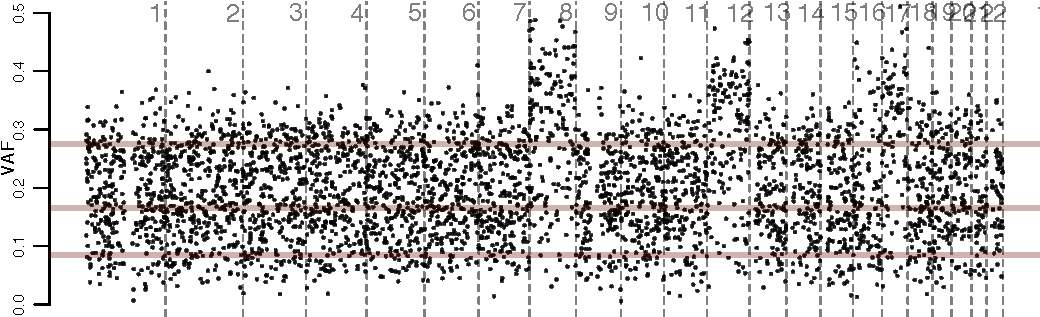
\includegraphics{src_guide_files/figure-latex/fig6-1} 

}

\caption{\label{fig6} Illustrate the effect of copy number on mutation VAF}\label{fig:fig6}
\end{figure}

On the previous figure, we see that for the lost chromosomes, because
there are now relatively more copies of sequenced DNA bearing the
mutations falling in those regions, the VAF is higher.

The mutation copy number of a given SNV is computed as:

\[ mutcopynumber=\frac{VAF}{\rho}(\rho N_{tumour} + (1-\rho) N_{normal})\]

Where \(N_{tumour}\) is the number of DNA copies in the tumour. In our
sample, \(\rho\) equals 0.55. Let's look at mutations in 1+0 tumour
regions (1 copy of the major, 0 copies of the minor). If their VAF is
around 0.4 as in the figure, their mutation copy number is
\[\frac{0.4}{0.55}(1\times0.55+2\times0.45)\approx
                                1\].

The mutation copy number is an estimate of the multiplicity, which is an
integer representing the number of bearing DNA copies bearing the
mutation. Dividing the mutation copy number by the multiplicity gives
the CCF: \[CCF=\frac{mutcopynumber}{multiplicity}\]

Most clustering method infer the multiplicity and then the CCF, and for
this, DPClust uses a preprocessing package
\href{https://github.com/Wedge-Oxford/dpclust_smchet_docker/blob/master/dpclust3p_v1.0.6.tar.gz}{dpclust3p}.

We will now run the main function of this package on our data.

\begin{Shaded}
\begin{Highlighting}[]
\NormalTok{lociFile  <-}\StringTok{ "loci.txt"}
\NormalTok{vcfFile <-}\StringTok{ "input/perfect_T2.T.128X_noXY.vcf"}
\NormalTok{subcloneFile <-}\StringTok{ "input/T2-128X_refit_subclones_noXY.txt"}
\NormalTok{alleleCountsFile <-}\StringTok{ "alleleCountsFile.txt"}
\NormalTok{cellFile <-}\StringTok{ "input/T2-128X_refit_cellularity_ploidy.txt"}
\NormalTok{rhoPsiFile <-}\StringTok{ "rhoPsiFile.txt"}
\NormalTok{rhopsip <-}\StringTok{ }\KeywordTok{read.table}\NormalTok{(cellFile,}\DataTypeTok{header=}\NormalTok{T)}
\NormalTok{dpInputFile <-}\StringTok{ "dpInput.txt"}
\KeywordTok{writeRhoPsi}\NormalTok{(rhopsip[}\DecValTok{1}\NormalTok{],rhopsip[}\DecValTok{2}\NormalTok{],rhopsip[}\DecValTok{3}\NormalTok{])}
\KeywordTok{createAlleleCountsFile}\NormalTok{(}\DataTypeTok{vcfFile=}\NormalTok{vcfFile, }\DataTypeTok{isperfect=}\NormalTok{T, }\DataTypeTok{outfile=}\NormalTok{alleleCountsFile)}
\KeywordTok{library}\NormalTok{(GenomicRanges)}
\KeywordTok{library}\NormalTok{(dpclust3p)}
\KeywordTok{suppressWarnings}\NormalTok{(}\KeywordTok{runGetDirichletProcessInfo}\NormalTok{(}\DataTypeTok{loci_file=}\NormalTok{lociFile,}
                                            \DataTypeTok{allele_frequencies_file=}\NormalTok{alleleCountsFile,}
                                            \DataTypeTok{cellularity_file=}\NormalTok{rhoPsiFile,}
                                            \DataTypeTok{subclone_file=}\NormalTok{subcloneFile,}
                                            \DataTypeTok{gender=}\StringTok{"male"}\NormalTok{,}
                                            \DataTypeTok{SNP.phase.file=}\StringTok{"NA"}\NormalTok{,}
                                            \DataTypeTok{mut.phase.file=}\StringTok{"NA"}\NormalTok{,}
                                            \DataTypeTok{output_file=}\NormalTok{dpInputFile))}
\end{Highlighting}
\end{Shaded}

Let's have a look at the results, especially the mutation copy number
vs.~the copy number. In this sample, the multiplicities cannot be
greater than 1, because there are no gained copy number.

\begin{figure}

{\centering 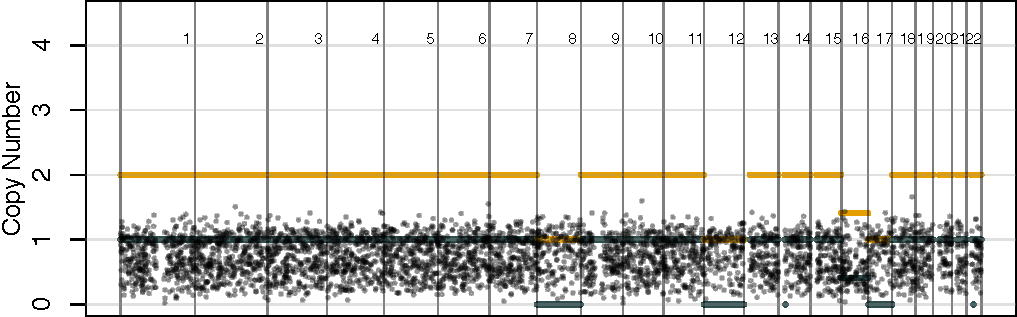
\includegraphics{src_guide_files/figure-latex/fig7-1} 

}

\caption{\label{fig7} Mutation copy number vs. DNA copy number.}\label{fig:fig7}
\end{figure}

Because we have that \(CCF=\frac{mutcopynumber}{multiplicity}\), in this
sample, where \(multiplicity=1\), \(CCF=mutcopynumber\).

Let's look at the distribution of CCF of mutations in non-subclonal copy
number segments.

\begin{figure}

{\centering 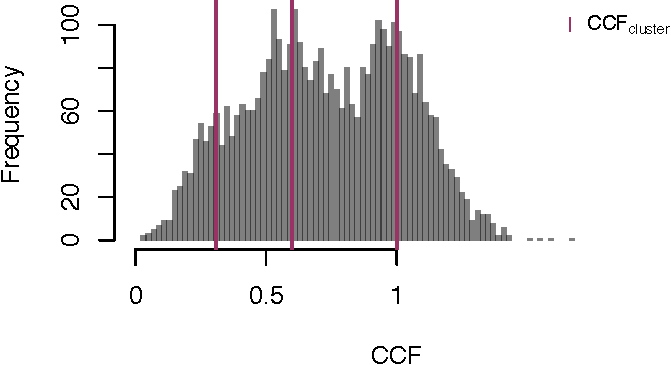
\includegraphics{src_guide_files/figure-latex/fig8-1} 

}

\caption{\label{fig8} Distribution of CCF. Vertical lines indicate the expected CCF of the clones.}\label{fig:fig8}
\end{figure}

This looks like an easy clustering task, which is expected since the
depth of coverage is so high.

\hypertarget{clustering}{%
\subsubsection{Clustering}\label{clustering}}

DPClust is a clustering method that allows to automatically find the
size, the number and the location of clusters of mutations at the same
CCF value. It was first described by Nik-Zainal and colleagues
(Nik-Zainal et al. 2012). We will now run DPClust on the mutations,
after integrating them with the Battenberg copy number profiles.

Next we run DPClust on the dpclust input file that we generated. This
file contains all the necessary information for DPClust to run.

An important aspect of DPClust is that it has strong default prior on
the concentration parameter, which will impact on the
concentration/number of clusters. Not all methods put a strong prior on
this parameter and allow for it to be influenced by the underlying data.
We will try and run DPClust with different values of this parameter.

The DPClust R package used here can be downloaded from
\href{https://github.com/Wedge-Oxford/dpclust_smchet_docker/blob/master/dpclust_v2.2.5.tar.gz}{\textbf{github}}.
DPClust has several dependencies, and there is a
\href{https://github.com/Wedge-Oxford/dpclust_smchet_docker/blob/master/Dockerfile}{\textbf{Docker}}
file available to install DPClust and all its dependencies. If you have
already installed R, the following packages are required:

\begin{quote}
BiocManager::install(c(``VariantAnnotation'',
``mcclust'',``KernSmooth'',``ks'',``lattice'',
``ggplot2'',``gridExtra'',``reshape2''))
\end{quote}

\begin{Shaded}
\begin{Highlighting}[]
\CommentTok{## load DPClust}
\KeywordTok{library}\NormalTok{(DPClust)}
\CommentTok{## load the data}
\NormalTok{cellularity <-}\StringTok{ }\KeywordTok{read.table}\NormalTok{(}\StringTok{"input/T2-128X_refit_cellularity_ploidy.txt"}\NormalTok{,}\DataTypeTok{header=}\NormalTok{T)[,}\StringTok{"cellularity"}\NormalTok{]}
\NormalTok{conc_param <-}\StringTok{ }\FloatTok{0.01}
\NormalTok{dataset  <-}\StringTok{  }\KeywordTok{load.data}\NormalTok{(dpInputFile, }
                       \DataTypeTok{cellularity=}\NormalTok{cellularity, }
                       \DataTypeTok{Chromosome=}\StringTok{"chr"}\NormalTok{, }
                       \DataTypeTok{position=}\StringTok{"end"}\NormalTok{,}
                       \DataTypeTok{WT.count=}\StringTok{"WT.count"}\NormalTok{, }
                       \DataTypeTok{mut.count=}\StringTok{"mut.count"}\NormalTok{, }
                       \DataTypeTok{subclonal.CN=}\StringTok{"subclonal.CN"}\NormalTok{, }
                       \DataTypeTok{no.chrs.bearing.mut=}\StringTok{"no.chrs.bearing.mut"}\NormalTok{, }
                       \DataTypeTok{mutation.copy.number=}\StringTok{"mutation.copy.number"}\NormalTok{, }
                       \DataTypeTok{subclonal.fraction=}\StringTok{"subclonal.fraction"}\NormalTok{, }
                       \DataTypeTok{phase=}\StringTok{"phase"}\NormalTok{,}
                       \DataTypeTok{is.male=}\NormalTok{T,}
                       \DataTypeTok{is.vcf=}\NormalTok{F,}
                       \DataTypeTok{ref.genome.version=}\StringTok{"hg19"}\NormalTok{,}
                       \DataTypeTok{min.depth=}\DecValTok{1}\NormalTok{,}
                       \DataTypeTok{min.mutreads=}\DecValTok{0}\NormalTok{,}
                       \DataTypeTok{supported_chroms=}\KeywordTok{as.character}\NormalTok{(}\DecValTok{1}\OperatorTok{:}\DecValTok{22}\NormalTok{))}
\CommentTok{## run DPClust}
\NormalTok{clustering  <-}
\StringTok{    }\KeywordTok{DirichletProcessClustering}\NormalTok{(}\DataTypeTok{mutCount=}\NormalTok{dataset}\OperatorTok{$}\NormalTok{mutCount, }
                               \DataTypeTok{WTCount=}\NormalTok{dataset}\OperatorTok{$}\NormalTok{WTCount, }
                               \DataTypeTok{no.iters=}\DecValTok{1250}\NormalTok{, }
                               \DataTypeTok{no.iters.burn.in=}\DecValTok{250}\NormalTok{, }
                               \DataTypeTok{cellularity=}\NormalTok{cellularity, }
                               \DataTypeTok{totalCopyNumber=}\NormalTok{dataset}\OperatorTok{$}\NormalTok{totalCopyNumber, }
                               \DataTypeTok{mutation.copy.number=}\NormalTok{dataset}\OperatorTok{$}\NormalTok{mutation.copy.number,}
                               \DataTypeTok{copyNumberAdjustment=}\NormalTok{dataset}\OperatorTok{$}\NormalTok{copyNumberAdjustment, }
                               \DataTypeTok{mutationTypes=}\NormalTok{dataset}\OperatorTok{$}\NormalTok{mutationType,}
                               \DataTypeTok{samplename=}\StringTok{"T2"}\NormalTok{, }
                               \DataTypeTok{subsamplesrun=}\KeywordTok{c}\NormalTok{(),}
                               \DataTypeTok{output_folder=}\StringTok{"./output_0.01"}\NormalTok{, }
                               \DataTypeTok{conc_param=}\NormalTok{conc_param, }
                               \DataTypeTok{cluster_conc=}\DecValTok{5}\NormalTok{,}
                               \DataTypeTok{mut.assignment.type=}\DecValTok{1}\NormalTok{,}
                               \DataTypeTok{most.similar.mut=}\OtherTok{NA}\NormalTok{,}
                               \DataTypeTok{min.frac.snvs.cluster=}\FloatTok{0.01}\NormalTok{, }
                               \DataTypeTok{max.considered.clusters=}\DecValTok{20}\NormalTok{)}
\KeywordTok{writeStandardFinalOutput}\NormalTok{(}\DataTypeTok{clustering=}\NormalTok{clustering, }
                         \DataTypeTok{dataset=}\NormalTok{dataset,}
                         \DataTypeTok{most.similar.mut=}\OtherTok{NA}\NormalTok{,}
                         \DataTypeTok{outfiles.prefix=}\StringTok{"output_0.01/T2-0.01"}\NormalTok{,}
                         \DataTypeTok{subsamplenames=}\KeywordTok{c}\NormalTok{(),}
                         \DataTypeTok{assign_sampled_muts=}\NormalTok{T,}
                         \DataTypeTok{write_tree=}\NormalTok{F)}
\end{Highlighting}
\end{Shaded}

Let's look at the results. DPClust outputs a figure showing the location
and size of the identified clusters in the CCF space.

\begin{figure}[H]
  \centering
  \includegraphics{output_0.01/T2_DirichletProcessplot_with_cluster_locations_2.png}
  \caption{\textbf{DPClust main output figure for single sample.}
  The histogram of the CCF values is shown and the location and
  density distribution of the clusters inferred by DPClust is shown on top.}
  \label{Figure6}
\end{figure}

It looks like DPClust has found an extra cluster between the two
subclones, and a substantial proportion of the clonal mutations have
been assigned to subclones.

Next we will first try running DPClust with a different concentration
parameter (from 0.01 we change it to 1).

\begin{figure}[H]
  \centering
  \includegraphics{output_1.00/T2_DirichletProcessplot_with_cluster_locations_2.png}
  \caption{\textbf{DPClust main output figure for single sample (concentration parameter x100).}
  The histogram of the CCF values is shown and the location and
  density distribution of the clusters inferred by DPClust is shown on top.}
  \label{Figure7}
\end{figure}

In this solution, we can see two very closeby clusters, which, if they
were real, would need to be linear due to the pigeonhole principle.
Rather arbitrarily, we tend to merge together clusters that are too
close in CCF space. In single-sample studies, they do not add much,
besides, we do not think that we have the power to distinguish between
those. Similarly we remove clusters that are \emph{too small} (e.g.
\textless{}50 mutations or \textless{}1\% of mutation load) as well as
superclonal clusters.

Thus, if we were to use this concentration parameter (1), the solution
is actually pretty good after merging and removing of the small cluster.
The true number of clusters, their CCF and associated number of SNVs
are:

\begin{longtable}[]{@{}lcr@{}}
\toprule
Subclone & CCF & N SNV\tabularnewline
\midrule
\endhead
1 & 1.00 & 2100\tabularnewline
2 & 0.60 & 1650\tabularnewline
3 & 0.31 & 600\tabularnewline
\bottomrule
\end{longtable}

In the previous run, DPClust has identified 3 clusters:

\begin{longtable}[]{@{}lcr@{}}
\toprule
Subclone & CCF & N SNV\tabularnewline
\midrule
\endhead
1 & 1.01 & 1787\tabularnewline
2 & 0.62 & 1706\tabularnewline
3 & 0.27 & 491\tabularnewline
\bottomrule
\end{longtable}

This is not far from the truth. What about mutation assignment? We can
see that there are less mutations that have been clustered than there
are in the design. This is partly because a few mutations are removed
and re-assigned posthoc, so they are present in the assignment files,
and partly because mutations with 0 alternate read counts are not
present in the truth file at all. Let's have a look at the contigency
table of assignment.

\begin{Shaded}
\begin{Highlighting}[]
\KeywordTok{kable}\NormalTok{(contingency_table,}\StringTok{"latex"}\NormalTok{, }\DataTypeTok{booktabs=}\NormalTok{T) }\OperatorTok
\StringTok{    }\KeywordTok{kable_styling}\NormalTok{(}\DataTypeTok{position=}\StringTok{"center"}\NormalTok{) }\OperatorTok
\StringTok{    }\KeywordTok{add_header_above}\NormalTok{(}\KeywordTok{c}\NormalTok{(}\StringTok{""}\NormalTok{,}\StringTok{"Truth"}\NormalTok{=}\DecValTok{4}\NormalTok{))}
\end{Highlighting}
\end{Shaded}

\begin{table}[H]
\centering
\begin{tabular}{lrrrr}
\toprule
\multicolumn{1}{c}{} & \multicolumn{4}{c}{Truth} \\
\cmidrule(l{3pt}r{3pt}){2-5}
  & 1 & 2 & 3 & NA\\
\midrule
2 & 9 & 95 & 403 & 0\\
3 & 5 & 159 & 58 & 0\\
4 & 231 & 1075 & 38 & 0\\
5 & 1642 & 127 & 8 & 0\\
NA & 19 & 18 & 9 & 0\\
\bottomrule
\end{tabular}
\end{table}

In the DPClust predictions, some mutations were not assigned to any
cluster, usually because they did not fall on any copy number segments.
The clustering contigency table looks relatively good, but this is not
unexpected as such high depth. With such prediction, we can start
characterising mutational signatures clonal vs.~subclonal, and between
subclone.

Now let's talk about the phylogeny.

\newpage

\hypertarget{phylogenetic-tree}{%
\subsubsection{Phylogenetic tree}\label{phylogenetic-tree}}

\hypertarget{single-sample-tree}{%
\paragraph{Single-sample tree}\label{single-sample-tree}}

Once the clustering of SNVs is obtained, the tree building can start.
Some methods have part or whole of the following process built in. For
example DPClust can take phasing of mutation as input to infer linear
vs.~branching subclones.

But here, we go through this step manually. Often the tree building from
single samples is rather uninformative.

There are few observations that can help disambiguate the phylogenetic
relationship (i.e.~linear vs.~branching) between subclones:

\begin{itemize}
\item{linear relationship}
  \begin{itemize}
 \item{the pigeonhole principle: the sum of ccfs of branching
     subclones at same tree height should be <=100\% of the ccf of
     their most recent common ancestor. Indeed if it was >100\%, this
     would mean that at least a few cells carry the same set of
     mutations. However, according to the infinite sites hypothesis, the same set of random mutations is highly
     unlikely to happen twice by chance alone. Therefore the
     smaller subclone must be a descendant of the bigger subclone.}
 \item{phasing of two mutations assigned to different clusters A and B, resp. If two
     mutations are present on the same read pair, they must have been
     present in the same cell. This means that at least one cell of subclone A and
     one cell of subclone B carried the same mutation. Moreover, under
     the infinite site hypothesis, each mutation appeared only once,
     hence, subclone A and B must be linearly related. }
 \end{itemize}
\item{branching relationship}
  \begin{itemize}
  \item{two significantly mutually exclusive mutations on haploid
      regions that are assigned to different clusters. On a clonally haploid
      region of the genome (i.e. 1 copy of allele A and 0 copies of
      allele B), only one copy of the genome is left to be
      mutated in cancer cells. Given two mutations assigned to two linear subclones,
      located in this haploid region and close to each other (distance
      below the read length), it is expected that the
      reads carrying the mutation of the smaller subclone should carry
      the mutation of the larger subclone. If these two mutations are
      mutually exclusive, they must belong to branching subclones.}
  \end{itemize}
\end{itemize}

In our sample, there is no way to know if the two subclones are linear
or branching. The sum of their \(CCF_{subcloneA}+CCF_{subcloneB}<1\), so
it could be both linear or branching. Usually, it is easier to call
linear than branching. But, if looking at mutation phasing in haploid
regions only, the proportion of linear vs.~branching subclone can be
compared.

\hypertarget{note-on-multi-sample-tree}{%
\paragraph{Note on multi-sample tree}\label{note-on-multi-sample-tree}}

With DPClust, multi-sample trees are also derived mostly manually. The
clustering process generalises trivially to multiple dimensions, and the
same code can be used to load the mutations from multiple samples.

An important step is to make sure the union of all mutations across
samples has been \emph{genotyped} if not called in all of them. Indeed,
mutations called in a given sample might have been missed in another
although the alternate read count is positive, i.e.\(VAF>0\). It is thus
important to rederive the alternate and reference counts for all
mutations in all samples before the clustering.

\newpage

\hypertarget{conclusion}{%
\section{Conclusion}\label{conclusion}}

In this guide, we have reviewed the steps of SRC one-by-one, running
them on a simulated tumour for which we know the underlying phylogeny
and subclonal structure. This has helped gain insight into the
practicalities behind SRC.

We have seen that mutation callers can include false positives at low
VAF, as well as false negatives. Copy number calling is ambiguous
because the ploidy can always be doubled to fit the data to integers and
manual refitting, which is often arbitrary, needs to be performed.
Unless given the ploidy experimentally (here we know it from the truth
design), there is little way to be sure about the fit. There are hints
in the data that can help diagnose bad copy number fits, for example
wrong purity can be seen when reconstructing the CCF of SNVs and the
highest peak is not at CCF=1 (i.e.~the peak of clonal mutation).

We have illustrated the impact of read depth on the VAF distribution and
CNA calling.

We have shown how some parameters of the clustering method can be
tweaked to lead to slightly different results, especially the
concentration parameter in DPClust, which can lead to different number
of clusters and reconstruction.

Altogether, single-sample-based SRC is not very informative about the
phylogeny and a lot of the sources of noise and ambiguities, such as
clustering of mutation and inferring phylogenetic relationships, can be
largely reduced using multi-sample strategies.

Unfortunately, multi-sample strategies are not always possible but
single-sample studies remain informative about the subclonality of
mutations and especially targetable drivers, their associated mutation
processes and the timing of the MRCA.

Once the subclonal strucutre is obtained, post-hoc assignment of other
types of variants, such as indels and structural variants can be
performed. Methods such as
\href{https://github.com/gerstung-lab/MutationTimeR}{\textbf{MutationTimer}}
are designed to do this (Gerstung et al. 2020).

\newpage

\hypertarget{references}{%
\section*{References}\label{references}}
\addcontentsline{toc}{section}{References}

\hypertarget{refs}{}
\leavevmode\hypertarget{ref-cibulskis_sensitive_2013}{}%
Cibulskis, Kristian, Michael S. Lawrence, Scott L. Carter, Andrey
Sivachenko, David Jaffe, Carrie Sougnez, Stacey Gabriel, Matthew
Meyerson, Eric S. Lander, and Gad Getz. 2013. ``Sensitive Detection of
Somatic Point Mutations in Impure and Heterogeneous Cancer Samples.''
\emph{Nature Biotechnology} 31 (3): 213--19.
\url{https://doi.org/10.1038/nbt.2514}.

\leavevmode\hypertarget{ref-dentro_portraits_2018}{}%
Dentro, Stefan C., Ignaty Leshchiner, Kerstin Haase, Maxime Tarabichi,
Jeff Wintersinger, Amit G. Deshwar, Kaixian Yu, et al. 2018. ``Portraits
of Genetic Intra-Tumour Heterogeneity and Subclonal Selection Across
Cancer Types.'' \emph{bioRxiv}, May, 312041.
\url{https://doi.org/10.1101/312041}.

\leavevmode\hypertarget{ref-dentro_principles_2017}{}%
Dentro, Stefan C., David C. Wedge, and Peter Van Loo. 2017. ``Principles
of Reconstructing the Subclonal Architecture of Cancers.'' \emph{Cold
Spring Harbor Perspectives in Medicine} 7 (8).
\url{https://doi.org/10.1101/cshperspect.a026625}.

\leavevmode\hypertarget{ref-ewing_combining_2015}{}%
Ewing, Adam D., Kathleen E. Houlahan, Yin Hu, Kyle Ellrott, Cristian
Caloian, Takafumi N. Yamaguchi, J. Christopher Bare, et al. 2015.
``Combining Tumor Genome Simulation with Crowdsourcing to Benchmark
Somatic Single-Nucleotide-Variant Detection.'' \emph{Nature Methods} 12
(7): 623--30. \url{https://doi.org/10.1038/nmeth.3407}.

\leavevmode\hypertarget{ref-gerstung_evolutionary_2020}{}%
Gerstung, Moritz, Clemency Jolly, Ignaty Leshchiner, Stefan C. Dentro,
Santiago Gonzalez, Daniel Rosebrock, Thomas J. Mitchell, et al. 2020.
``The Evolutionary History of 2,658 Cancers.'' \emph{Nature} 578 (7793):
122--28. \url{https://doi.org/10.1038/s41586-019-1907-7}.

\leavevmode\hypertarget{ref-howie_flexible_2009}{}%
Howie, Bryan N., Peter Donnelly, and Jonathan Marchini. 2009. ``A
Flexible and Accurate Genotype Imputation Method for the Next Generation
of Genome-Wide Association Studies.'' \emph{PLOS Genet} 5 (6): e1000529.
\url{https://doi.org/10.1371/journal.pgen.1000529}.

\leavevmode\hypertarget{ref-li_aligning_2013}{}%
Li, Heng. 2013. ``Aligning Sequence Reads, Clone Sequences and Assembly
Contigs with BWA-MEM.'' \emph{arXiv:1303.3997 {[}Q-Bio{]}}, May.
\url{http://arxiv.org/abs/1303.3997}.

\leavevmode\hypertarget{ref-nik-zainal_life_2012}{}%
Nik-Zainal, Serena, Peter Van Loo, David C. Wedge, Ludmil B. Alexandrov,
Christopher D. Greenman, King Wai Lau, Keiran Raine, et al. 2012. ``The
Life History of 21 Breast Cancers.'' \emph{Cell} 149 (5): 994--1007.
\url{https://doi.org/10.1016/j.cell.2012.04.023}.

\leavevmode\hypertarget{ref-salcedo_community_2020}{}%
Salcedo, Adriana, Maxime Tarabichi, Shadrielle Melijah G. Espiritu, Amit
G. Deshwar, Matei David, Nathan M. Wilson, Stefan Dentro, et al. 2020.
``A Community Effort to Create Standards for Evaluating Tumor Subclonal
Reconstruction.'' \emph{Nature Biotechnology} 38 (1): 97--107.
\url{https://doi.org/10.1038/s41587-019-0364-z}.

\leavevmode\hypertarget{ref-van_loo_allele-specific_2010}{}%
Van Loo, Peter, Silje H. Nordgard, Ole Christian Lingjærde, Hege G.
Russnes, Inga H. Rye, Wei Sun, Victor J. Weigman, et al. 2010.
``Allele-Specific Copy Number Analysis of Tumors.'' \emph{Proceedings of
the National Academy of Sciences} 107 (39): 16910--5.
\url{https://doi.org/10.1073/pnas.1009843107}.


\end{document}
